\newpage
\section{Metodologia Experimental}

\subsection{Materiais}
O material utilizado foi:
\begin{itemize}
\item Computador.
\item Software Orcad.

\end{itemize}
O experimento foi dividido em duas partes, sendo a parte 1 para o modulador série e a parte 2 com o modulador a diodo.

\subsubsection{Modulador série}
Para execução da parte 1 do experimento, faz-se necessário executar os seguintes passos (com base no circuito da figura \ref{f_sch_mod_am_serie}:

\begin{itemize}
\item montar o circuito mostrado na figura \ref{f_sch_mod_am_serie} no software Orcad;
\item utilizar um sinal senoidal de 200Hz (2 $V_{pp}$) como modulante e um sinal de 100kHz como portadora;
\item Obter o índice de modulação $\gamma$ do circuito através do método 1 e do método 2;
\item verificar quais são os limites para $\gamma$;
\item caso seja possível obter índice m > 1,observe o que ocorre com sinal quando se utiliza o método 2. É possível aplicar este método na avaliação de índices de modulação maiores que 100%?;
\item determinar o fator de mérito do modulador, utilizando como carga um resistor de 10 M$\Omega$ e um capacitor de 20pF, simulando a ponta de prova do osciloscópio.
\item analisar o sinal de saída no domínio da frequência;
\item como é possível reduzir eventuais componentes de frequência espúrias à saída?
\end{itemize}

\begin{figure}[H]
\centering
\caption{Modulador série.}
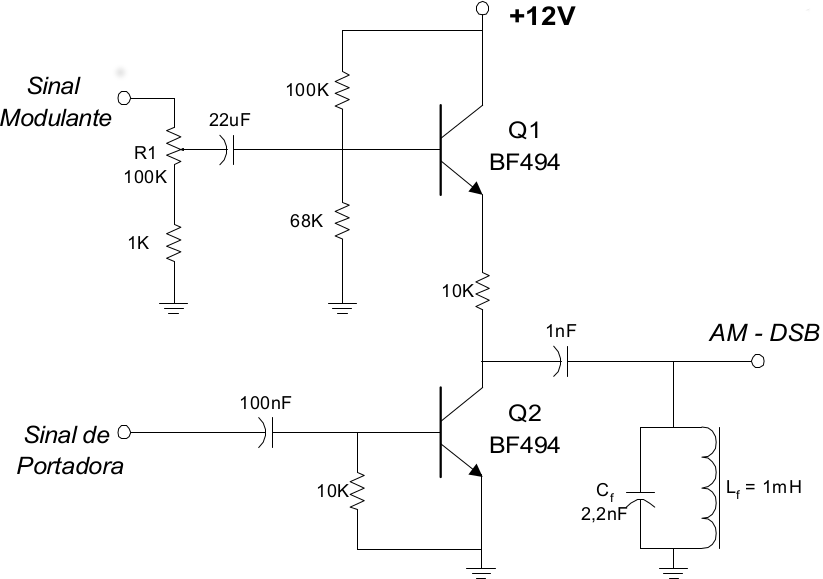
\includegraphics[scale=0.4]{Imagens/sch_mod_am_serie.png}
\label{f_sch_mod_am_serie}
\end{figure}

\subsubsection{Modulador a diodo}
Para execução da parte 2 do experimento, faz-se necessário executar os seguintes passos (com base no circuito da figura \ref{f_sch_mod_am_diodo}):

\begin{itemize}
\item montar o circuito mostrado na figura \ref{f_sch_mod_am_diodo} no software Orcad;
\item utilizar um sinal senoidal de 2kHz (2 $V_{pp}$) como modulante e um sinal de 100kHz (5 $V_{pp}$) como portadora;
\item calcular o valor de $L_1$ e $C_1$ de modo que a frequência de ressonância fique próxima de $f_c$.
\item verificar se o sinal modulante é banda estreita;
\item Obter o índice de modulação $\gamma$ do circuito através do método 1 e do método 2;
\item caso seja possível obter índice m > 1,observe o que ocorre com sinal quando se utiliza o método 2. É possível aplicar este método na avaliação de índices de modulação maiores que 100%?;
\item determinar o fator de mérito do modulador, utilizando como carga um resistor de 10 M$\Omega$ e um capacitor de 20pF, simulando a ponta de prova do osciloscópio.
\item analisar o sinal de saída no domínio da frequência;
\end{itemize}

\begin{figure}[H]
    \centering
    \caption{Modulador a diodo.}
    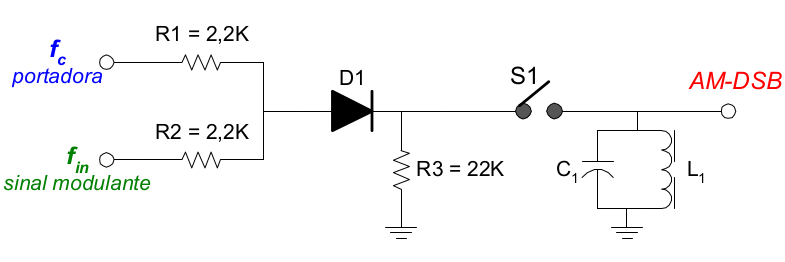
\includegraphics[scale=0.5]{Imagens/sch_mod_am_diodo.png}
    \label{f_sch_mod_am_diodo}
\end{figure}
